%%%%%%%%%%%%%%%%%%%%%%%%
%% Sample use of the infthesis class to prepare a thesis. This can be used as 
%% a template to produce your own thesis.
%%
%% The title, abstract and so on are taken from Martin Reddy's csthesis class
%% documentation.
%%
%% MEF, October 2002
%%%%%%%%%%%%%%%%%%%%%%%%

%%%%
%% Load the class. Put any options that you want here (see the documentation
%% for the list of options). The following are samples for each type of
%% thesis:
%%
%% Note: you can also specify any of the following options:
%%  logo: put a University of Edinburgh logo onto the title page
%%  frontabs: put the abstract onto the title page
%%  deptreport: produce a title page that fits into a Computer Science
%%      departmental cover [not sure if this actually works]
%%  singlespacing, fullspacing, doublespacing: choose line spacing
%%  oneside, twoside: specify a one-sided or two-sided thesis
%%  10pt, 11pt, 12pt: choose a font size
%%  centrechapter, leftchapter, rightchapter: alignment of chapter headings
%%  sansheadings, normalheadings: headings and captions in sans-serif
%%      (default) or in the same font as the rest of the thesis
%%  [no]listsintoc: put list of figures/tables in table of contents (default:
%%      not)
%%  romanprepages, plainprepages: number the preliminary pages with Roman
%%      numerals (default) or consecutively with the rest of the thesis
%%  parskip: don't indent paragraphs, put a blank line between instead
%%  abbrevs: define a list of useful abbreviations (see documentation)
%%  draft: produce a single-spaced, double-sided thesis with narrow margins
%%
%% For a PhD thesis -- you must also specify a research institute:
% \documentclass[phd,iccs,twoside]{infthesis}

%% For an MPhil thesis -- also needs an institute
% \documentclass[mphil,ianc]{infthesis}

%% MSc by Research, which also needs an institute
% \documentclass[mscres,irr]{infthesis}

%% Taught MSc -- specify a particular degree instead. If none is specified,
%% "MSc in Informatics" is used.
% \documentclass[msc,cogsci]{infthesis}
\documentclass[msc,ai]{infthesis}  % for the MSc in Informatics

%% Undergraduate project -- specify the degree course and project type
%% separately
% \documentclass[bsc]{infthesis}
% \course{Artificial Intelligence and Psychology}
% \project{Fourth Year Project Report}

%% Put any \usepackage commands you want to use right here; the following is 
%% an example:
\usepackage{natbib}
\usepackage{url}
% \usepackage{hyperref}

%% Information about the title, etc.
\title{Fast low-rank metric learning}
\author{Dan-Theodor Onea\c{t}\u{a}}

%% If the year of submission is not the current year, uncomment this line and 
%% specify it here:
% \submityear{1785}

%% Optionally, specify the graduation month and year:
% \graduationdate{February 1786}

%% Specify the abstract here.
\abstract{%
    This doctoral thesis will present the results of my work into the
    reanimation of lifeless human tissues.
}

%% Now we start with the actual document.
\begin{document}

%% First, the preliminary pages
\begin{preliminary}

%% This creates the title page
\maketitle

%% Acknowledgements
\begin{acknowledgements}
Many thanks to my mummy for the numerous packed lunches; and of course to
Igor, my faithful lab assistant.
\end{acknowledgements}

%% Next we need to have the declaration.
\standarddeclaration

%% Finally, a dedication (this is optional -- uncomment the following line if
%% you want one).
% \dedication{To my mummy.}

%% Create the table of contents
\tableofcontents

%% If you want a list of figures or tables, uncomment the appropriate line(s)
% \listoffigures
% \listoftables

\end{preliminary}

%%%%%%%%
%% Include your chapter files here. See the sample chapter file for the basic
%% format.

\chapter{Introduction}
\label{ch:introduction}

$k$ nearest neighbours ($k$NN) is one of the oldest and simplest classification methods. It has its origins in an unpublished technical report by \citet{fix1951} and since then it has become standard textbook material \citep{russell1996,mitchell1997,bishop2006}. In the last 50 years, $k$NN was present in most of the machine learning related fields (pattern recognition, statistical classification, data mining, information retrieval, data compression) and it plays a role in many applications (e.g., face recognition, plagiarism detection, vector quantization).

The idea behind $k$NN is intuitive and straightforward: classify a given point according to a majority vote of its neighbours; the selected class is the one that is the most represented amongst the $k$ nearest neighbours. This is easy to implement and it usually represents a good way to approach new problems or data sets. Despite its simplicity $k$NN is still a powerful tool, performing surprisingly well in practice \citep{holte1993}.

There are also other characteristics that make $k$NN an interesting method. First, $k$NN makes no assumptions about the underlying structure of the data. No a priori knowledge is needed beforehand, but we let the data ``speak for itself''. The accuracy increases with the number of points in the data set and, in fact, it approaches Bayes optimality as the cardinality of the training set goes to infinity and $k$ is sufficiently large \citep{cover1967}. Second, $k$NN is able to represent complex functions with non-linear decision boundaries by using only simple local approximations.
% (this behaviour is hardly captured by any parametric method). 
Lastly, $k$NN operates in a ``lazy'' fashion. The training data set is just stored and its use is delayed until testing. The quasi-inexistent training
%\footnote{There can be a training step in which the parameter $k$ is tuned via cross-validation or we can we imagine different technique being applied for dimensionality reduction}
 allows the easy addition of new training examples. 

$k$NN has some drawbacks that influence both the computational performance and the quality of its predictions. Since $k$NN has to store all the exemplars, the memory requirements are directly proportional with the number of instances in the training set. The cardinality of the data also influences the method's speed. All computations are done at testing time, making $k$NN painfully slow when applied on large data sets. 
%The cost of classification is also linear in the cardinality of the training set because all the computations are done at testing. and it is often prohibitive for large data sets. 

The accuracy of $k$NN is closely related to how we define what ``close'' and ``far'' mean for our data set and task. Mathematically, the notion of dissimilarity is incorporated into $k$NN by using different distance metrics. Usually the standard Euclidean metric is not satisfactory and the aim is to find the particular metric that gives the best results on our data set for a given task (section~\ref{sec:theoretical-background}).
%However, more important are the issues related to the accuracy. On one hand, there is not clear how we should choose a dissimilarity metric and how notions as ``close''/``far'' are defined for our data set. This is non-trivial and usually the standard Euclidean metric is not satisfactory (see Subsection \ref{subsec:distance-metrics}, for a more detailed discussion). On the other hand, there  
%All these problems are even more acute nowadays when we have to operate on huge sets of data with many attributes (e.g., images, videos, DNA sequences, etc.). 
There is an entire literature that tries to come up with possible solutions (section~\ref{sec:related-methods}).

\section{Neighbourhood component analysis}
\label{sec:nca}
 
This thesis focuses on neighbourhood component analysis (NCA; \citealp{goldberger2004}). The NCA method learns the metric that maximizes the expected number of correctly classified points (section~\ref{sec:general-presentation}). Using the NCA metric with $k$NN usually improves the performance over simple $k$NN, since we use the label information to construct a suitable metric that selects the relevant attributes. 

NCA considers only a family of distance metrics known as Mahalanobis (or quadratic) metrics; these are characterized by having associated a linear transformation (section~\ref{sec:theoretical-background}). By restricting the transformation to be non-square we obtain the corresponding low-rank metric. Such a projection results in a low dimensional representation of the original data that reduces the storage needs and the computational expense at test time. Also it alleviates some of the concerns that have been raised regarding the usefulness of nearest neighbours methods for high dimensional data \citep{beyer1999, hinneburg2000}. The curse of dimensionality arises for $k$NN, because the distances become indiscernible for many dimensions. For a given distribution the maximum and the minimum distance between points become equal in the limit of many dimensions. 
NCA proves to be an elegant answer for the above issues and, consequently, it was successfully used in a variety of applications: face recognition \citep{butman2008}, hyper-spectral image classification \citep{weizman2007}, acoustic modelling \citep{singh2010} and even reinformcent learning \citep{keller2006}. 

However, the method introduces additional training time. The objective function needs the pairwise distances of the points, so the function evaluation is quadratic in the number of data points. Also the optimization process is iterative. For large data sets, NCA training becomes prohibitively slow. For example, \citet{weinberger2009} reported that the original implementation ran out of RAM and \citet{weizman2007} had to use only 10\% of their data set in order to successfully train the model. There is only little previous work that uses NCA for large scaled applications. One example is \citep{singh2010}, who parallelizes the computations across multiple computers and adopts various heuristics to prune terms of the objective function and the gradient.
%One elegant answer is provided by \citet{goldberger2004}. They proposed a new method, Neighbourhood Component Analysis (NCA), that copes with the drawbacks in a unified manner by learning a low-rank metric. This reduces both the storage and the computational cost, because the algorithm uses the data set projected into a lower subspace, with fewer attributes needed. Also the accuracy is improved, because the label information is used for constructing a proper metric that selects the relevant attributes. However, NCA introduces a consistent training time, because we now have an objective function whose gradient is quadratic in the number of data points that is optimized using iterative methods. 

\section{Reducing the computational cost}
\label{sec:reducing}

The main aim of this project is to reduce NCA training time without significant loses in accuracy (chapter \ref{ch:reducing}). We start our investigation with the most simple ideas: use only a subset of the data set (section \ref{sec:sub-sampling}) or train the metric on different mini-batches subsampled from the data set (section \ref{sec:mini-batches}). This last idea can be further refined by using clustered mini-batches. Also we present an alternative mini-batch algorithm (section \ref{sec:stochastic-learning}) that decreases the theoretical cost. 

These methods can achieve further speedings if we use approximations of the objective function. Simple approximation ideas (such as ignoring the points which are farther away than a certain distance from the current point) were mentioned in the original paper \citep{goldberger2004} and they are re-iterated by \citet{weinberger2007} and \citet{singh2010}. We present a more principled approach that borrows ideas from fast kernel density estimation problems \citep{deng1995,gray2003,gray2003b}. We first recast NCA into a class-conditional kernel density estimation framework (section \ref{sec:cc-kde}) and next we present how fast density estimation is done using a space partitioning structure, such as $k$-d trees (section \ref{sec:approximate}). Similar work of fast metric learning was done by \citep{weinberger2008} which uses ball trees \citep{omohundro1989} to accelerate a different distance metric technique, large margin nearest neighbour (LMNN; \citealp{weinberger2009}). However, LMNN is different from NCA and the way in which ball trees are applied also differs from our approach.
%$k$-d trees \citep{bentley1975} group together near points and can be used to quickly select only those points that have significant contribution. These sort of  have been successfully applied for speeding up $k$NN at query time \citep{friedman1977} and we will use them in a similar manner for NCA's testing operations. 

An alternative for the approximation method is to change the model such that it allows exact and efficient computations. In the kernel density estimation model, we can use compact support kernels instead of the standard Gaussian functions. The expense is reduced because only the points that lie in the compact support are used for estimating the density (section \ref{sec:exact-computations}).

We evaluate the proposed techniques in terms of accuracy and speed  (chapter \ref{ch:evaluation}). Also we provide low dimensional representations of the projected data. The results are promising, showing that we can obtain considerable speed-ups for large data sets while retaining almost the same accuracy as in the classic case. For small and medium sized data sets the accuracy and the time spent are similar to the standard NCA.

%, we could interpret NCA as a class-conditional kernel-density estimate and then use different types of kernels instead of the Gaussian ones; we will focus especially on kernels with compact support, because they do not introduce approximation errors and computations can be done more efficiently than in the previous case. 

% \chapter{Background}

This chapter sets the theoretical basis for the following discussion on low-rank metrics. We start with a brief mathematical introduction into distance metrics. Then we outline the characteristics of the Mahalanobis-like metric. At the end of the chapter we review some of the most prominent work in the area. The method we study, neighbourhood component analysis (NCA), is presented in chapter \ref{ch:nca}.

\section{Theoretical background}
\label{sec:theoretical-background}
  A distance metric is a mapping from a pair of inputs to a scalar. Let $d(x,y)$ denote the distance function between the arguments $x$ and $y$. Given a set $\mathcal{S}$, we say that $d$ is a metric on $\mathcal{S}$ if it satisfies the following properties for any $x,y,z\in\mathcal{S}$:
	\begin{itemize}
		\item Non-negativity: $d(x,y) \ge 0$.
		\item Distinguishability: $d(x,y)=0 \Leftrightarrow  x\equiv y$.
		\item Symmetry: $d(x,y)=d(y,x)$.
		\item Triangle Inequality: $d(x,y)\leq d(x,z) + d(z,y)$.
	\end{itemize}
	
	A metric can be defined on any set~$\mathcal{S}$ of objects. The distance metric is valid as long as the above properties hold for any elements in the set. However, for the scope of our applications we limit ourselves to points in $D$ dimensional real space. The inputs will be represented by column vectors $\xB,\yB \in \mathbb{R}^D$. In this case the distance $d$ is a function from $\mathbb{R}^D\times\mathbb{R}^D$ to $\mathbb{R}$. A well known example of such a function is the Euclidean metric. This is defined by:
	\begin{align}
		 d(\mathbf{x},\mathbf{y}) = \sqrt{(\mathbf{x-y})\tr(\mathbf{x-y})}, \quad\mbox{with }\mathbf{x,y}\in \mathbb{R}^D.
	\end{align}
	
Albeit useful in many scenarios, the Euclidean metric has two properties that are problematic in machine learning applications \citep{dwinnell-online}:
	\begin{description}
		 \item[Sensitivity to variable scaling.]{ In geometrical situations, the values across all $D$ dimensions are measured in the same unit of length. In practical situations however, each dimension encodes a different feature of the data set. The Euclidean metric is sensitive to scaling and it returns different results if we change the measurement units for one of the $D$ variables. We compensate for these differences by dividing the values on dimension~$i$ by the standard deviation~$s_i$ on that direction:
		  \begin{align}
		   d(\mathbf{x},\mathbf{y}) &= \sqrt{\left(\frac{x_1-y_1}{s_1}\right)^2+\cdots+\left(\frac{x_D-y_D}{s_D}\right)^2} = \notag\\
		   &= \sqrt{(\mathbf{x-y})\tr\SB^{-1}(\mathbf{x-y})}, \label{eq:new-distance}
		  \end{align}
		 where $\SB=\operatorname{diag}(s_1^2,\cdots,s_D^2)$ and $s_i^2 = \operatorname{var}[x_i],\forall i=1,\cdots,D$.
		 }
		 \item[Invariance to correlated variables.] {Euclidean distance does take into account any associations between variables. We can take into account the correlations between attributes if we replace $\SB$ in equation \eqref{eq:new-distance} with the covariance matrix of the data:
		 \begin{align}
		 d(\mathbf{x},\mathbf{y}) = \sqrt{(\mathbf{x-y})\tr\SB^{-1}(\mathbf{x-y})},
		 \label{eq:mahalnobis-distance}
		 \end{align}
		 where $\SB = \operatorname{cov}[\mathcal{D}]$, $\mathcal{D}$ is the dataset. The metric defined in equation \eqref{eq:mahalnobis-distance} is known as the Mahalanobis distance. %This is an extended version of the Euclidean metric which takes into account the correlation in the data.
		 }
	\end{description}
%A distance metric represents a function or a mapping from a pair of inputs to a scalar proportional to the dissimilarity of the inputs. Additionally, in order to be a proper distance, the given function ought to be non-negative, symmetric and it should respect the triangle inequality. The most common and used metric is the standard Euclidean distance. It often appears and is very useful in many geometrical situations, when distances between points need to be calculated. However, it has two major drawbacks that are problematic especially in machine learning applications. First of all, Euclidean distance is sensitive to scaling. Whilst in mathematical problems this does not constitute an issue, in real situations, we may have features that are measured in different units (e.g., seconds, kilograms, etc.) and we will obtain different distances between our data points if we change the scalings on some axis. The other problem is the fact that it does not take into consideration the correlations in the data structure. It can often happen that more attributes reflect the same information present in the data and, consequently, the distance is strongly influenced by those attributes. Take the example of face recognition: there the pixels from the image background are highly correlated and they usually reflect the same information, i.e., the colour of the background.

%The standard notation is $d(\mathbf{x},\mathbf{y})$ and it represents a function that calculates the distance between two inputs $\mathbf{x}$ and $\mathbf{y}$ (column vectors in a $D$ dimensional space $\mathbf{x},\mathbf{y}\in \mathbb{R}^D$). Essentially, the metric maps a pair from $\mathbb{R}^D\times \mathbb{R}^D$ to a real number scalar. 

%Formally, $d:\mathbb{R}^D\times \mathbb{R}^D \to \mathbb{R}$ is a metric if for any $\mathbf{x,y,z}\in \mathbb{R}^D$ the following properties hold: %\cite{Kochanski2009}
%\begin{itemize}
% \item Non-negativity: $d(\mathbf{x},\mathbf{y}) \ge 0$.
% \item Distinguishability: $d(\mathbf{x},\mathbf{y})=0 \Leftrightarrow  \mathbf{x}=\mathbf{y}$.
% \item Symmetry: $d(\mathbf{x},\mathbf{y})=d(\mathbf{y},\mathbf{x})$.
% \item Triangle Inequality: $d(\mathbf{x},\mathbf{y})\leq d(\mathbf{x},\mathbf{z}) + d(\mathbf{z},\mathbf{y})$.
%\end{itemize}

%Now we can relate the previous definition with the most common and used example: Euclidean distance. This is defined as:
%\begin{align}
% d_E(\mathbf{x},\mathbf{y}) = \sqrt{(\mathbf{x-y})^T(\mathbf{x-y})}, \mbox{ with }\mathbf{x,y}\in \mathbb{R}^D.
%\end{align}

%Unfortunately, the Euclidean distance has two major drawbacks that are problematic especially in machine learning applications\footnote{\url{http://matlabdatamining.blogspot.com/2006/11/mahalanobis-distance.html}}:
%\begin{itemize}
% \item{ \textbf{Sensitivity to variable scaling}. In geometrical situations, all variables are measured in the same units of length; for some of the real data variability is stronger on certain dimensions than on others. Naturally, we try to compensate the acute difference; so we want components with high variability to receive less weight than those with low variability. We can obtain this by simply rescaling the components with corresponding values $(s_i)_{i=\overline{1,D}}$: 
%  \begin{align}
%   d(\mathbf{x},\mathbf{y}) &= \sqrt{\left(\frac{x_1-y_1}{s_1}\right)^2+\cdots+\left(\frac{x_D-y_D}{s_D}\right)^2} = \notag\\
%   &= \sqrt{(\mathbf{x-y})^TS^{-1}(\mathbf{x-y})} \label{eq:new-distance}
%  \end{align}
% where $S^{-1}=\operatorname{diag}(s_1^2,\cdots,s_D^2)$. 
% }
% \item{ \textbf{Invariance to correlated variables}. Euclidean distance does not take into account the correlations in the data structure. For face images, for example, the pixels in the background, usually have the same colour, especially if they are close to each other; if these pixels differ strongly for other picture of the same person, we will be heavily penalized, because their number is large and the distance will be influenced by them. Therefore, we should not take into account all these variables since they reflect the same information (i.e., the color of the background). Intuitively, we want our distance metric to reflect the correlation in the data. This can be easily achieved by replacing $S$ in Equation \eqref{eq:new-distance} with the covariance matrix of the data.
% \begin{align}
% d(\mathbf{x},\mathbf{y}) = \sqrt{(\mathbf{x-y})^TS^{-1}(\mathbf{x-y})}, \mbox{ with } S = \operatorname{cov}(\mathcal{X})
% \label{eq:mahalnobis-distance}
% \end{align}
% where $\mathcal{X}$ is the dataset $\mathcal{X}=(\mathbf{x}_i)_{i=\overline{1,N}}$. 
% }

	\begin{figure}
		 \centering
			  \subfigure[Face recognition]{\label{fig:face-recog}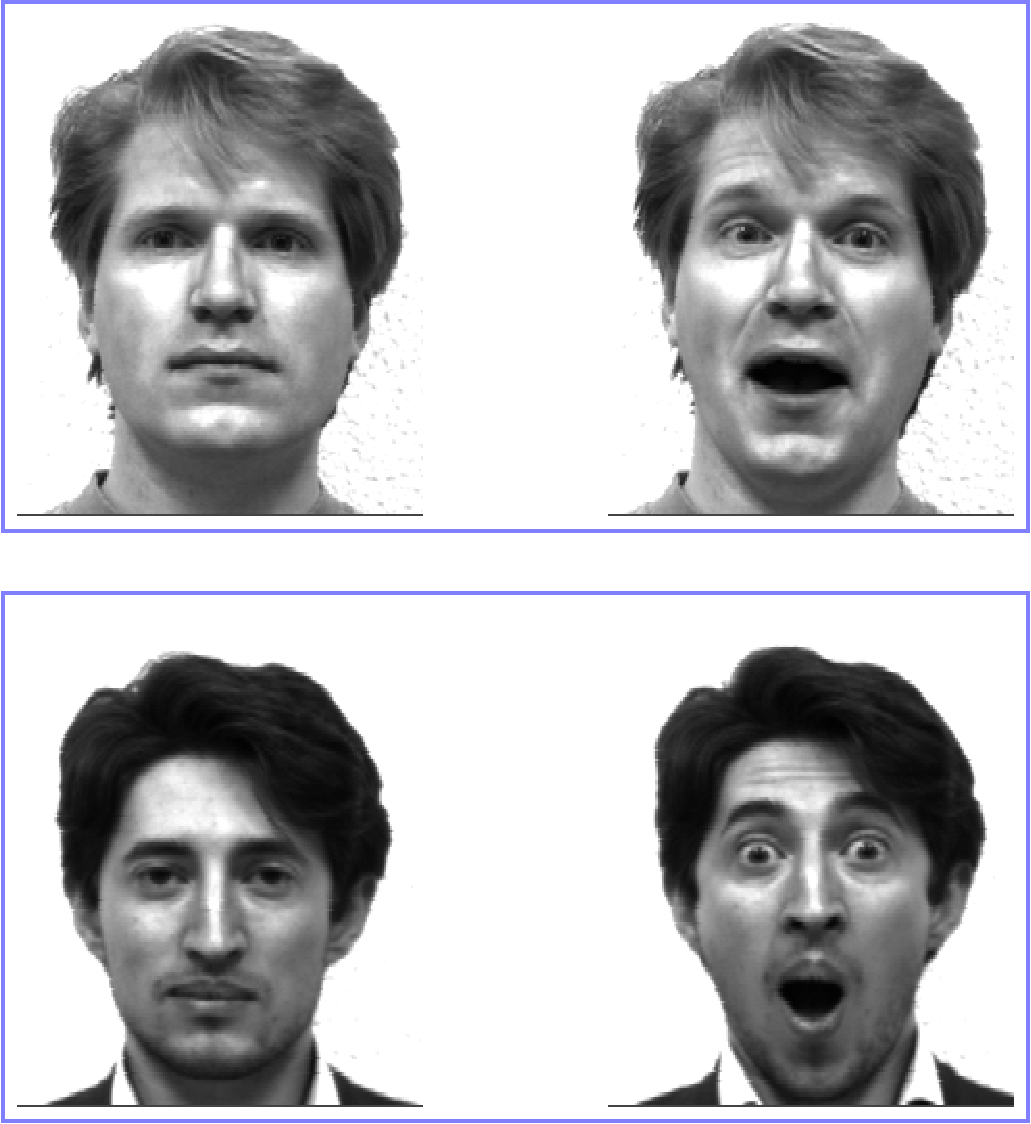
\includegraphics[width=0.4\textwidth]{images/face-recog}}
			    \hspace{0.07\textwidth}
			 \subfigure[Expression recogntion]{\label{fig:expression-recog}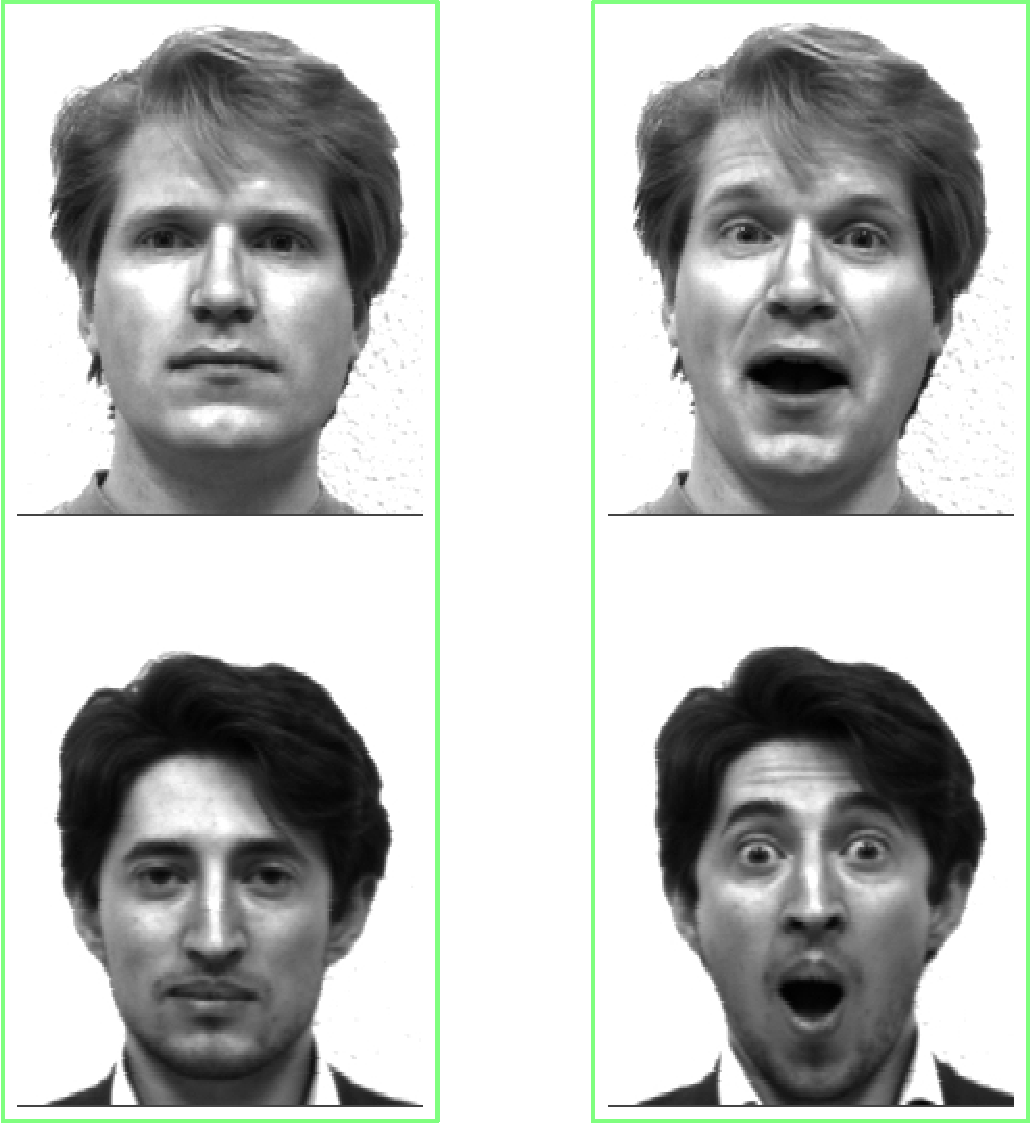
\includegraphics[width=0.4\textwidth]{images/expression-recog}}
		\caption[Motivating the need for a distance metric --- different tasks are solved by different metrics]{On a given data set we might need to perform multiple tasks; in this example: face recognition and expression recognition. The Euclidean metric is not optimal since we want different pairs of equivalence for the two tasks. A good distance metric should be task dependent. These images are an extract from Yale face database.}
		\label{fig:face-recog-vs-expression-recog}
	\end{figure}

The Mahalanobis metric extends the Euclidean distance by incorporating data specific information. But a good metric should be even more flexible than that. Apart from the data set, we are also given a task to perform. We want our metric to extract and discriminate only between information that is relevant to our given task. Take the example of images and face recognition. The pixels from the image background are highly correlated and they reflect the same information: the colour of the background. If the two pictures of the same subject have different backgrounds, we get a high distance between the images. Since we are not interested at all in
the background colour, the metric should identify all the pixels in the background as non-relevant and down-weight their importance. In figure \ref{fig:face-recog-vs-expression-recog}, we illustrate why we need our metric should depend on a given task and why for a given data set it is not optimal to use a fixed metric.

We can further generalize the result from equation \eqref{eq:mahalnobis-distance}.
Instead of setting $\SB$ as the covariance of the data, we let $\SB$ be a different matrix. The problem of determining a suitable matrix
$\SB^{-1}$ is called Mahalanobis (or quadratic) distance metric learning. We note that $\SB^{-1}$ ought to be positive semi-definite $\mathbf{x}\tr\SB^{-1}\mathbf{x} \geq 0, \forall\;\mathbf{x}$. This ensures that the norm is a real value: $d(\mathbf{x},\mathbf{0})\equiv\lVert \mathbf{x}\lVert = \sqrt{\mathbf{x}\tr\SB^{-1}\mathbf{x}}\in\mathbb{R}$.

%We need to further extend the previous result. Given a data set we usually do not care for the data set variance, but want to adapt the weights on the dimensions such that they suit our task. When we want to discriminate among face, we have some dimensions that 

%Equation \eqref{eq:mahalnobis-distance} is the standard definition of the Mahalanobis distance. Since we do not care for any variance in the data, but just for that is representative for our particular task (as discussed in Section \ref{sec:introduction}), we will consider different matrices $S$ that are suitable for the given query. Since we want our metric to discriminate among faces, we down-weight the less informative dimensions. 

\begin{figure}
		 \centering
			  \subfigure[Mahalanobis metric in the original space]{\label{fig:mahalanobis}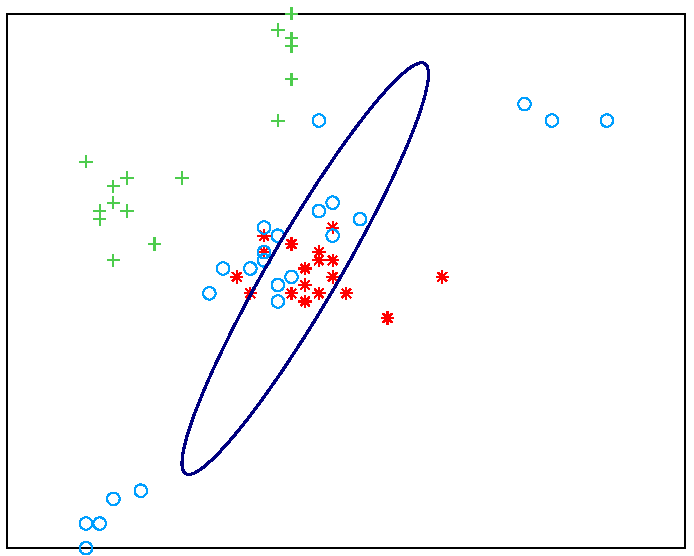
\includegraphics[width=0.45\textwidth]{images/mahalanobis}}
			    \hspace{0.02\textwidth}
			 \subfigure[Euclidean metric in the projected space]{\label{fig:euclidean}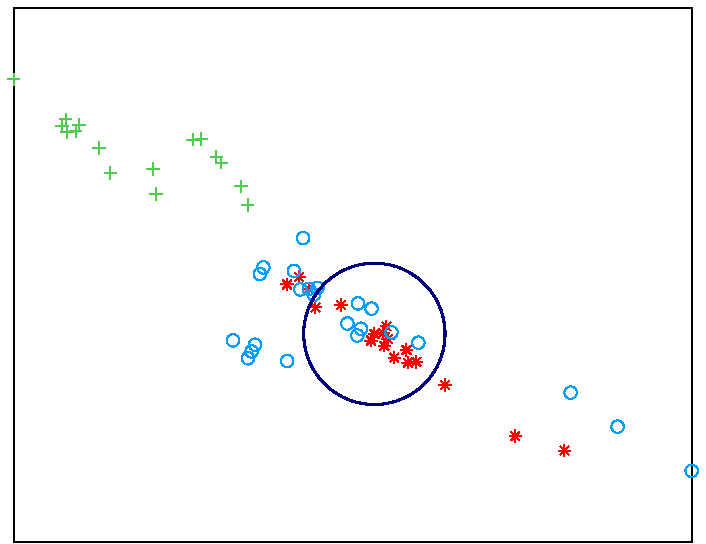
\includegraphics[width=0.45\textwidth]{images/euclidean}}
		\caption[Equivalence between the Mahalanobis metric and its associated linear projection]{Illustration of the equivalence between a Mahalanobis metric in the original data space and an Euclidean metric in the transformed data space. The metrics are denoted by an ellipse and, respectively, a circle whose contours indicate equal distance from the centre point to the rest of the points.}
		\label{fig:mahalanobis-euclidean}
	\end{figure}

There is an interesting equivalence between a Mahalanobis-like metric and a linear transformation. Using the Cholesky decomposition or other matrix square root we can write $\SB^{-1}=\AB\tr\AB$, which gives $\lVert \mathbf{x} \lVert = \sqrt{(\AB\mathbf{x})\tr(\AB\mathbf{x})}$, where $\AB$ represents a linear transformation of the data. Hence, the problem of finding a suitable distance metric $\SB$ is equivalent to the problem of finding a good linear transformation $\AB$ and then applying Euclidean distance in the projected space (figure \ref{fig:mahalanobis-euclidean}). We will discuss these two variants interchangeably and we will often parametrize our models in terms of $\AB$.

\section{Related methods}
\label{sec:related-methods}

The first attempts in metric learning were simple alterations of the Euclidean metric to improve $k$NN performance. For example, \citet{mitchell1997} suggests weighting each attribute of the data points such that the cross validation error is minimized. This technique is equivalent to stretching the axis of the relevant attributes and compressing the axis of the attributes that are less informative. The approach is a special case of learning a diagonal metric, equation \eqref{eq:new-distance}. Another method \citep{moore1994} is to eliminate the least relevant attributes: they are given a weight of zero. Albeit useful, these techniques are restrictive as the feature scaling does not reflect how the data covary.

\citet{hastie1996} proposed discriminant adaptive nearest neighbours (DANN), a method that constructs a local metric for each particular query. The metric is chosen such that it provides the best discrimination amongst classes in the neighbourhood of the query point. This increases the already costly testing time of $k$NN. However, DANN method provides a non-linear metric if we take into account all the possible resulting local linear distance metrics. Even though non-linear transformations are an interesting domain, we will concentrate our attention on linear metrics as they are less prone to over-fitting and easier to learn and represent.

\citet{xing2003} proposed learning a Mahalanobis-like distance metric for clustering in a semi-supervised context. There are specified pairs of similar data points and the algorithm finds the linear projection that minimizes the distance between these pairs without collapsing the whole data set to a single point. This approach is formulated as a convex optimization problem with constraints. The solution is attained using an iterative procedure, such as Newton-Raphson. This method assumes that the underlying density of the data is unimodal which leverages the assumption-free $k$NN. Another drawback is the training time, because the iterative process is costly for large data sets.

Relevant component analysis (RCA; \citealp{bar2003, shental2002}) is another method that makes use of the labels of the classes in a semi-supervised way to provide a distance metric. More precisely, RCA the so-called chunklet information. A chunklet contains points from the same class, but the class label is not known; data points that belong to the same chunklet have the same label, while data points from different chunklets do not necessarily belong to different classes. The main idea behind RCA is to find a linear transformation which ``whitens'' the data with respect to the averaged within-chunklet covariance matrix \citep{weinberger2009}. Compared to the method of \citet{xing2003}, RCA has the advantage of presenting a closed form solution, but it has even stricter assumptions about the data: it assumes that the data points in each class are normally distributed so they can be described using only second order statistics \citep{goldberger2004}.

Large margin nearest neighbour (LMNN; \citealp{weinberger2009}) is a metric learning method that was designed especially for $k$NN classification. LMNN has some similar characteristics to the support vector machine (SVM) technique. As SVM, LMNN brings together points from the same class trying to separate the classes by a certain margin. Also LMNN inherits the convexity property and can be optimize as a semi-definite programming. \citet{weinberger2008} worked on fast metric learning by introducing ball trees to speed up the computations. In \citep{weinberger2008}, they extended LMNN to learn local metrics further improving its performance.

Metric learning is an ongoing research area in machine learning with an abundance of different techniques. For a good report that covers many related methods, the reader is referred to \citep{yang2006}.

%% ... etc ...

%%%%%%%%
%% Any appendices should go here. The appendix files should look just like the
%% chapter files.
%\appendix
%\include{appendix1}
%% ... etc...

%% Choose your favourite bibliography style here.
\bibliographystyle{apalike}

%% If you want the bibliography single-spaced (which is allowed), uncomment
%% the next line.
\singlespace

%% Specify the bibliography file. Default is thesis.bib.
\bibliography{thesis}

%% ... that's all, folks!
\end{document}
